\documentclass[9pt]{extarticle}
\usepackage{amsmath}
\usepackage{bm}
\usepackage{graphicx}
\usepackage[utf8]{inputenc}
\usepackage{caption}
\usepackage{subcaption}
\title{Modeling a synaptic transmission, \\
Mathematical modeling}
\author{Group 9; \\
Student \# 732064, 732095, 732078, 723818, 723980 }

\begin{document}
\maketitle

\documentclass{article}
\usepackage{amsmath}
\usepackage{bm}
\usepackage{graphicx}
\usepackage[utf8]{inputenc}
\usepackage{caption}
\usepackage{subcaption}
\title{Modeling a synaptic transmission, \\
Mathematical modeling}
\author{Student numbers }


\begin{document}
\maketitle


\section{Introduction}
%We chose project 1. Our focus was making numerical solvers for the problem in all dimensions, and putting som boundary conditions on the edges to estimate the time for the signalt to transmitt. We also modeled the time using what we have learned for matematical modeling. \\
We tried to find the time estimate for the signal to be transmitted in several different ways. 
A good way to start was by finding a time 	scale. 


In this report, we start by showing a Monte Carlo simulation of random walk as a first model for the diffusion of the neurotransmitters.  Next, modeling equations are derived for the initial model, as well as the expanded model which includes the glia cells.  After this, mathematical modeling is used to obtain a rough estimate of the time used to transmit a signal. This is followed by several attempts at solving a 1D model of the problem, and then a 2D model.



\begin{thebibliography}{9}
%\cite[p. 34]{holstad}%
\bibitem{holstad}
  Jörg Henrik Holstad,
  \emph{Modellering av Diffusjon av Nevrotransmittere
i den Ekstracellulære Væsken}.
  2011.\\
https://www.duo.uio.no/bitstream/handle/10852/10871/MasteroppgaveHenrikHolstad.pdf
Retrieved 13.11.2014
\end{thebibliography}
\end{document}

% simulations:
\documentclass{article}
\usepackage{amsmath}
\usepackage{bm}
\usepackage{graphicx}
\usepackage[utf8]{inputenc}
\usepackage{caption}
\usepackage{subcaption}
\title{Simulating a synaptic cleft using monte carlo methods}
\author{Jon Christian Halvorsen }


\begin{document}
\maketitle

\section*{Simulating a synaptic transmission using monte carlo methods}

Since this project involves solving a lot of equations, and solving equations is a lot of hard work, we'll preliminary just try our hands on doing some simulations. We're doing a monte carlo simulation of diffusion in a cubic room scaled to represent a synaptic cleft. We release 5000 neurotransmitters in the middle of one side (wall $a$) and apply a brownian motian to each of the particles, thereby watching how it unfolds.

In the simplest version we just scattered the neurotransmitters, confirming that they scatter nearly uniformly out in each 3 dimensions.

The next step would be to lock all the elements inside a box (setting the flux out to zero) and implementing the dendrite wall with receptors. We call the dendrite wall $c$, opposite end of       $a$. We then assume:
\begin{itemize}
\item The probability of a neurotransmitter binding with a receptor is dependent on the distance from the dendrite wall (wall c) and how many of the receptors are already taken.
\item The probability of a neurotransmitter disconnecting from the receptor is also quantifiable so we can get some form of equilibrium  (at least when all the walls are closed).
\end{itemize}

Implementing this is also rather straightforward. As a last step we factor in the process of clearing the cleft after the signal is sent. We assume:
\begin{itemize}
\item There exists GLIA-cells in walls $b$ and $d$.
\item The two last walls are for now free, but have no flux out of them.
\item The probability for a neurotransmitter to bind to a GLIA-cell is dependent on the distance to the cell.
\item We also have a probability of "unbonding" with the GLIA-cell, and when we are the neurotransmitter is marked as inactive.
\item All inactive neurotransmitters have a probability (dependent on distance) of going back into the axon, thus clearing the synaptic cleft one particle at the time.
\item The probability of leaving the axon as an inactive neurotransmitter is equal to zero.
\item 
\end{itemize}


\end{document}



% theory:


\section{Deriving the modeling equations}
\subsection*{Diffusion equation}
Given the equations from the task \cite{task}, we quickly conclude that the diffusion of the neurotransmitters can be modeled by
\begin{align}
\label{eq:diffusion}
\frac{dc}{dt} &= \kappa \nabla^2 c \\
\label{eq:BC}
\nabla c \cdot n &= g(t,c),
\end{align}
with the last equation being the Neumann boundary condition. In the equations, $c$ is the concentration of neurotransmitters, $\kappa$ is the diffusion constant and $g(t,c)$ is a boundary flux.


\subsection{The binding process}
First we look at the reversible chemical reaction
\begin{align}
\label{eq:boundNeurotransmitter}
\text{R} + \text{N} \rightleftharpoons \text{RN},
\end{align}
where R is the number of receptors and N is the number of neurotransmitters.
The reaction rates are $k_1$ to the right and $k_2$ to the left, being respectively the probability for the reactions to occur in their direction. 
We get 3 ODE's from this chemical reaction:
\begin{align*}
\frac{d[\text{R}]}{dt} &= -k_1[\text{R}][\text{N}] + k_2[\text{RN}]\\
\frac{d[\text{N}]}{dt} &= -k_1[\text{R}][\text{N}] + k_2[\text{RN}]\\
\frac{d[\text{RN}]}{dt} &= k_1[\text{R}][\text{N}] - k_2[\text{RN}],
\end{align*}
where [R], [N] and [RN] are the concentrations of the receptors, neurotransmitters and the bound product of them.
We may consider [N][R] the probability of a neurotransmitter meeting an unoccupied receptor, and $k_1$ the probability of the binding reaction happening. Likewise for $k_2$. Next, we insert $c$ for $[\text{N}]$.  Introducing $P^R$ as the probability of a receptor being unoccupied, and $(1-P^R)$ as the probability that the neurotransmitter is attached to the receptor leads to the following simplification \cite{holstad} 
of the above ODE's:
\begin{align}
\label{eq:changeInConcentration}
\frac{dc}{dt} &= -k_1cP^R + k_2(1-P^R)\\
\label{eq:changeInPR}
\frac{dP^R}{dt} &= -k_1cP^R + k_2(1-P^R).
\end{align}

\subsection{Glia cells}
\begin{align*}
\text{T} + \text{N} \rightleftharpoons \text{TN} \rightarrow \text{N}_{\text{inactive}} + \text{T}.
\end{align*}
Here, we define $k_3, k_4, k_5$ as the reaction rates of first rightward, first leftward, second rightward reactions.

Similarly to the binding process, we get the following set of equations:
\begin{align*}
\kappa \nabla c \cdot n &= -k_3c P^T + k_4(1-P^T)\\
\frac{dP^T}{dt} &= -k_3c P^T + (1-P^T)(k_4 + k_5).\\
\end{align*}
Combining these equations, we get
\begin{align*}
\kappa \nabla c \cdot n &= -c(k_1 P^R + k_3 P^T) + k_2 (1-P^R) + k_4 (1-P^T)    \\
\frac{dP^R}{dt} &= -ck_1 P^R + k_2(1-P^R)\\
\frac{dP^T}{dt} &= -ck_3 P^T + (k_4 + k_5)(1-P^T).\\
\end{align*}


\section{Modeling a time scale}
We wanted to find a scaling for time in order to get a feel about the time it takes before a signal is transmitted. In order to do that, we use the diffusion equation
\begin{align}
\label{diffusion_unscaled}
\frac{\partial c^{*}}{\partial t^{*}} = \kappa \nabla^2 c^{*}.
\end{align}
Since we were given a radius and a height, we chose to use cylindrical coordinates. Thus $\nabla^2$ becomes
$$ \nabla^2 f = \frac{1}{r^{*}} \frac{\partial}{\partial r^{*}} \Big( r^{*} \frac{\partial f}{\partial r^{*}} \Big) +\frac{1}{(r^{*})^2}\frac{\partial^2 f}{\partial \phi^2} + \frac{\partial^2 f}{\partial (z^{*})^2}. $$
We scale the equation so that
$$\begin{array}{lr}
c^{*} &= Cc\\ r^{*} &=Rr\\ z^{*} &= Lz\\ t^* &=Tt.\\
\end{array}$$
With the scaling, the equation becomes
$$\frac{\partial Cc}{\partial Tt} = \kappa \Bigg( \frac{1}{Rr} \frac{\partial }{\partial Rr} \Big( Rr \frac{\partial Cc}{\partial Rr} \Big) +\frac{1}{(Rr)^2}\frac{\partial^2 Cc}{\partial \phi^2} + \frac{\partial^2 Cc}{\partial (Lz)^2} \Bigg). $$
We assume that the neurotransmitters are released in the centre of the axon. Due to rotational symmetry, $c$ becomes independent of $\phi$. Since $R >> h$, it follows that $1/R^2<<1/L^2$, and we assume $1/R^2 \approx 0$. After these simplifications the equation becomes
$$\frac{1}{T} \frac{\partial c}{\partial t} = \kappa  \frac{1}{L^2}\frac{\partial^2 c}{\partial z^2} . $$
To simplify, we set all derivatives to be $ \sim 1 $, and obtain
$$\frac{1}{T}  = \kappa \frac{1}{L^2}.  $$
Solving for $T$ gives us a timescale
$$T = \frac{L^2}{\kappa} = \frac{(15\cdot 10^{-9}\text{m})^2}{0.3\cdot 10^{-12} \text{m$^2$/s}} = 0.75 \text{ms}. $$
This is by no means a correct time for the signal to be transmitted, but we could guess that the real time will be of order $1 \text{ms}$.


% id implementations:
\section{1D Model}

Let us look at the easiest possible model of the synaptic cleft; a 1D model. Assume the neurotransmitters diffuse along a line, released from the axon terminal and arriving at the dendritic spine. When the neurotransmitters attach and detach to the receptors, we model it as a total flux $J$ of neurotransmitters leaving or entering the domain. Further, we assume that when the neurotransmitters are within a small distance $\epsilon$ of the dendritic spine, they are close enough to react with the receptors.

The number of receptors on one membrane is R $\approx \gamma_R \cdot \pi r^2 \approx 152$, where $\gamma_R$ is the density of receptors and $r$ is the radius of the synaptic cleft \cite{task}. N $= 5000$ as before. Let $\Omega$ be the line between $0$ and $L$.

Now, look at the area near the dendritic spine. Let $\Omega_{\epsilon}$ be a small area close to $L$ with width $\epsilon$, see Figure \ref{fig:model_1d}. Let $\gamma_{N\epsilon}(t)$ be the density of neurotransmitters in $\Omega_{\epsilon}$, $\gamma_R$ the density of receptors in the area $\epsilon$, and $P^R(t)$ be the probability that one receptor is available. With reaction constants $k_1$ and $k_2$, the flux can be expressed as

\begin{align*}
J(t) = k_1 \gamma_{N\epsilon}(t) \gamma_R P^R(t) - k_2 \gamma_R (1-P^R(t)).
\end{align*}


\begin{figure}[ht]
        \centering
        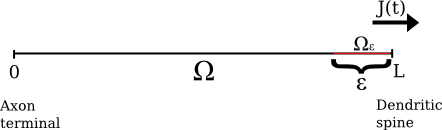
\includegraphics[clip=true,width=0.6\textwidth]{model_1d}
        \caption{Model of the synaptic cleft in one dimension}
        \label{fig:model_1d}
\end{figure}
\subsection{Initial values and boundary conditions}

Initial values:

\[ c(x,0) = \left\{ 
  \begin{array}{l l}
    \textrm{N} & \text{ if } x = 0\\
    0 & \text{ elsewhere}
  \end{array} \right.\]

Neumann boundary conditions:

\begin{align*}
c_x(0,t) &= 0, \\
c_x(L,t) &= J(t).
\end{align*}


The homogeneous Neumann boundary condition at $x = 0$ comes from the physical explanation that neurotransmitters cannot go back through the axon terminal.




\subsection{Scaling of variables}


We use the same scaling as in section 4 and replace in the unscaled diffusion equation (\ref{diffusion_unscaled}) such that

\begin{align*}
\frac{\textrm{N}}{T}\frac{\partial c}{\partial t} &= \kappa \frac{\textrm{N}}{L^2}\frac{\partial^2c}{\partial x^2} \Rightarrow
\frac{\partial c}{\partial t} = \eta \frac{\partial^2c}{\partial x^2}, & \eta = \kappa\frac{T}{L^2}.
\end{align*}

Using the values $L = 15 \cdot 10^{-9}$, $T = 10^{-3}$ and $\kappa = 0.3\cdot 10^{-12}$, we get the resulting value $\eta = 4/3$.




\subsection{Numerical scheme}

Using Crank-Nicholsons method, we obtain 

\begin{align*}
(1 - \frac{k}{2h^2} \delta^2_x)C^{n+1}_m = (1 + \frac{k}{2h^2} \delta^2_x) C_m^n,
\end{align*}

where $k$ and $h$ are the time and space steps, respectively. Adding Neumann boundary conditions to the system, we expand the numerical scheme to involve boundary points, and an additional term such that the resulting scheme becomes

\begin{align*}
\left(I - \frac{r}{2} A\right)C^{n+1} = \left(I + \frac{r}{2} A\right) C^n + \frac{k}{2}(d^n + d^{n+1}),
\end{align*}

where $r = \frac{k}{h^2}$,


\begin{align*}
A = 
\begin{pmatrix}
  -3/2h & 2h & -h/2 &  \\
  1 & -2 & 1 &  \\
  &  \ddots & \ddots & \ddots  \\
  &  & 1 & -2 & 1 \\
  &  & -3/2h & 2h & -1/2h 
\end{pmatrix} 
\textrm{, }
C = \begin{pmatrix}
C_0 \\
C_1 \\
\vdots \\
C_{M} \\
C_{M+1} 
\end{pmatrix}
\textrm{, }
d =
\begin{pmatrix}
0 \\
0 \\
\vdots \\
0 \\
J(t)
\end{pmatrix}.
\end{align*}

The result of this scheme is visualized in figure \ref{fig:model_1d_plot}. 


\begin{figure}[h!]
    \centering
    \begin{subfigure}[b]{0.45\textwidth}
        \centering
        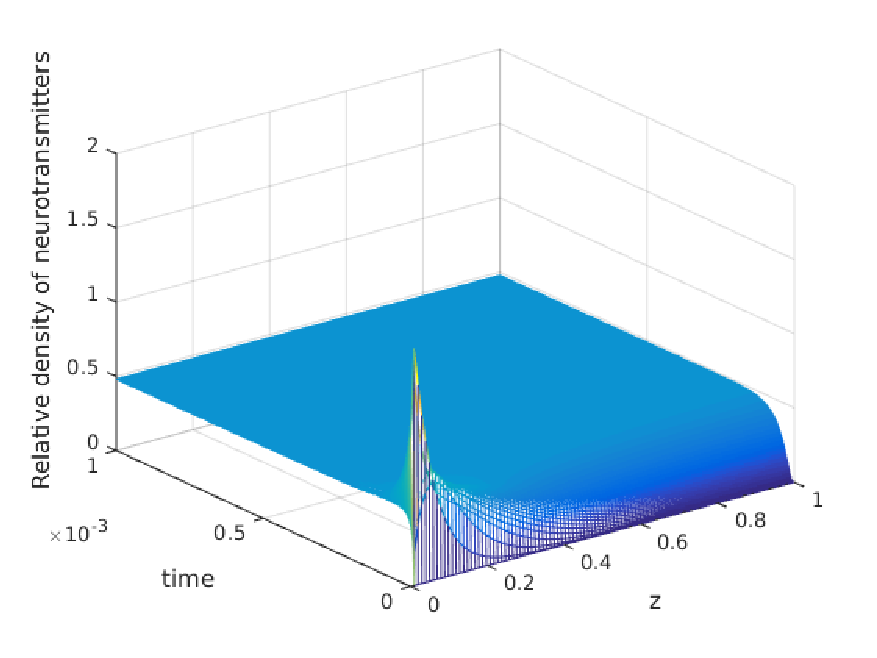
\includegraphics[width=\textwidth]{1dmodel_plot-crop}
        \caption{Distribution of neurotransmitters on a line over time. $k_1 = 10$, $k_2 = 1$, $\Delta t = 0.001$, $\Delta z = 0.01$.}
    \end{subfigure}%
    ~ 
    \begin{subfigure}[b]{0.45\textwidth}
        \centering
        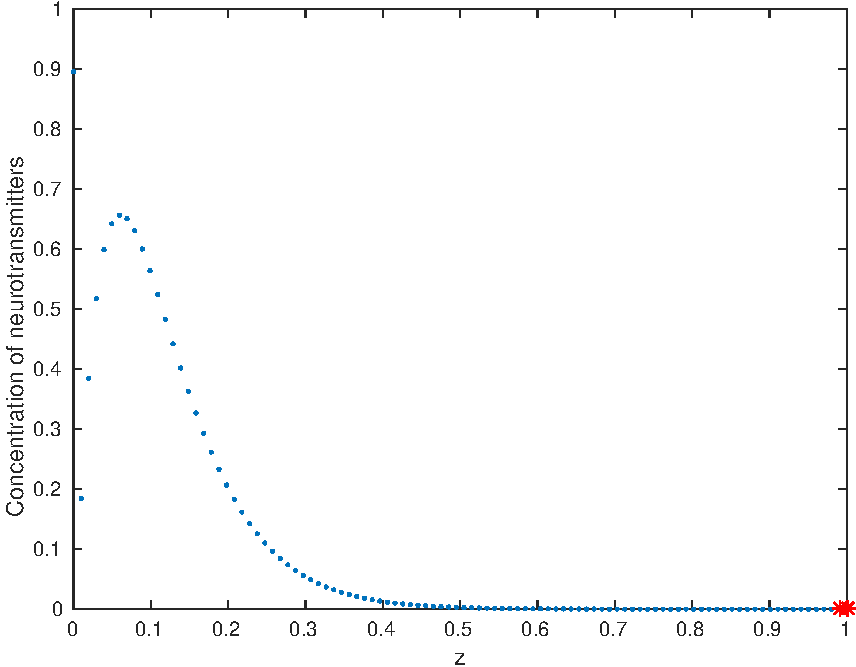
\includegraphics[width=\textwidth]{distribution_plot_1d-crop}
        \caption{Distribution of neurotransmitters on a line at a certain time. The red dots in the right corner marks $\Omega_{\epsilon}$.}
    \end{subfigure}
    \caption{Distribution of neurotransmitters on a line using the Matlab script $dim1.m$.}
    \label{fig:model_1d_plot}
\end{figure}
\documentclass[11pt, a4paper]{article}\usepackage[]{graphicx}\usepackage[]{color}
%% maxwidth is the original width if it is less than linewidth
%% otherwise use linewidth (to make sure the graphics do not exceed the margin)
\makeatletter
\def\maxwidth{ %
  \ifdim\Gin@nat@width>\linewidth
    \linewidth
  \else
    \Gin@nat@width
  \fi
}
\makeatother

\definecolor{fgcolor}{rgb}{0.345, 0.345, 0.345}
\newcommand{\hlnum}[1]{\textcolor[rgb]{0.686,0.059,0.569}{#1}}%
\newcommand{\hlstr}[1]{\textcolor[rgb]{0.192,0.494,0.8}{#1}}%
\newcommand{\hlcom}[1]{\textcolor[rgb]{0.678,0.584,0.686}{\textit{#1}}}%
\newcommand{\hlopt}[1]{\textcolor[rgb]{0,0,0}{#1}}%
\newcommand{\hlstd}[1]{\textcolor[rgb]{0.345,0.345,0.345}{#1}}%
\newcommand{\hlkwa}[1]{\textcolor[rgb]{0.161,0.373,0.58}{\textbf{#1}}}%
\newcommand{\hlkwb}[1]{\textcolor[rgb]{0.69,0.353,0.396}{#1}}%
\newcommand{\hlkwc}[1]{\textcolor[rgb]{0.333,0.667,0.333}{#1}}%
\newcommand{\hlkwd}[1]{\textcolor[rgb]{0.737,0.353,0.396}{\textbf{#1}}}%

\usepackage{framed}
\makeatletter
\newenvironment{kframe}{%
 \def\at@end@of@kframe{}%
 \ifinner\ifhmode%
  \def\at@end@of@kframe{\end{minipage}}%
  \begin{minipage}{\columnwidth}%
 \fi\fi%
 \def\FrameCommand##1{\hskip\@totalleftmargin \hskip-\fboxsep
 \colorbox{shadecolor}{##1}\hskip-\fboxsep
     % There is no \\@totalrightmargin, so:
     \hskip-\linewidth \hskip-\@totalleftmargin \hskip\columnwidth}%
 \MakeFramed {\advance\hsize-\width
   \@totalleftmargin\z@ \linewidth\hsize
   \@setminipage}}%
 {\par\unskip\endMakeFramed%
 \at@end@of@kframe}
\makeatother

\definecolor{shadecolor}{rgb}{.97, .97, .97}
\definecolor{messagecolor}{rgb}{0, 0, 0}
\definecolor{warningcolor}{rgb}{1, 0, 1}
\definecolor{errorcolor}{rgb}{1, 0, 0}
\newenvironment{knitrout}{}{} % an empty environment to be redefined in TeX

\usepackage{alltt}  
\usepackage[T1]{fontenc}               	% Vise norske tegn.
\usepackage[utf8]{inputenc}						% For ?f¥ kunne skrive norske tegn.
%\usepackage[norsk]{babel}								% Tilpasning til norsk.
\usepackage{graphicx}       						% For ?f¥ inkludere figurer.
\usepackage{subcaption}
\usepackage{amsmath,amssymb} 						% Ekstra matematikkfunksjoner.
\usepackage{indentfirst}                % For å få oppgaevbokstavene til å se pene ut
\usepackage{siunitx}							      % M?f¥ inkluderes for blant annet ?f¥ f?f¥ tilgang til kommandoen \SI (korrekte m?f¥ltall med enheter)
%\usepackage{textcomp}
%	\sisetup{exponent-product = \cdot}      % Prikk som multiplikasjonstegn (i steden for kryss).
% 	\sisetup{output-decimal-marker  =  {,}} % Komma som desimalskilletegn (i steden for punk
% 	\sisetup{separate-uncertainty = true}   % Pluss-minus-form p?f¥ usikkerhet (i steden for p
\usepackage{booktabs}                     % For ?f¥ f?f¥ tilgang til finere linjer (til bruk i tabeller og sli
\usepackage[font=small,labelfont=bf]{caption}	% For justering av figurtekst og tabelltekst.


% Disse kommandoene kan gj?f¸re det enklere for LaTeX ?f¥ plassere figurer og tabeller der du ?
\setcounter{totalnumber}{5}
\renewcommand{\textfraction}{0.05}
\renewcommand{\topfraction}{0.95}
\renewcommand{\bottomfraction}{0.95}
\renewcommand{\floatpagefraction}{0.35}
\newcommand{\tab}{\hspace*{2em}}
\renewcommand{\labelitemi}{$ $}



\author{Navn Navnesen}

\title{{\bf TMA4195} Mathematical Modelling Project}
\IfFileExists{upquote.sty}{\usepackage{upquote}}{}
\begin{document}

\maketitle

\section*{Deriving the modelling equations}
\subsection*{Diffusion equation}
Flux $J$:
\begin{align*}
J = -D\nabla c
\end{align*}


\begin{align*}
c_t = \kappa \Delta c\\
\frac{dc}{dt} = \kappa \nabla^2 c
\end{align*}
Neumann BC:
\begin{align*}
\nabla c \cdot n = g(t,c)
\end{align*}

\subsection*{The binding process}

First we look at the reversible chemical reaction

\begin{align*}
\text{R} + \text{N} \rightleftharpoons \text{RN}
\end{align*}

with reaction rate $k_1^*$ to the right and $k_2^*$ to the left, being respectively the probability for the reactions to occur in their direction. 
We get 3 ODE's from this chemical reaction:

\begin{align*}
\frac{d[\text{R}]}{dt} &= -k_1^*[\text{R}][\text{N}] + k_2^*[\text{RN}],\\
\frac{d[\text{N}]}{dt} &= -k_1^*[\text{R}][\text{N}] + k_2^*[\text{RN}],\\
\frac{d[\text{RN}]}{dt} &= k_1^*[\text{R}][\text{N}] - k_2^*[\text{RN}],
\end{align*}
where [R], [N] and [RN] are the concentratinos of the receptors, neurotransmitters and the bound product of them.
We may consider [N][R] the probability of a neurotransmitter meeting an unoccupied receptor, and $\bar{k}_1^*$ the probability of the binding reaction happening. Likewise for $\bar{k}_2^*$. $P^R$ is the probability of a receptor being unoccupied, $(1-P^R)$ the probability that the neurotransmitter is attatched to the receptor, leeds to the following simplification of the above ODE's:

\begin{align*}
\frac{d[\text{N}]}{dt} &= -\bar{k}_1^*[\text{N}]P^R + \bar{k}_2^*(1-P^R),\\
\frac{dP^R}{dt} &= -\bar{k}_1^*[\text{N}]P^R + \bar{k}_2^*(1-P^R).\\
\end{align*}

If we assume that the receptors are not uniformly distributed, we need to introduce a $\gamma(x)$ to describe the density of receptors.
At the boundary:
\begin{align*}
\frac{d[\text{N}]}{dt} &= -\bar{k}_1^*[\text{N}]\gamma P^R + \bar{k}_2^*\gamma(1-P^R),\\
\frac{dP^R}{dt} &= -\bar{k}_1^*[\text{N}]\gamma P^R + \bar{k}_2^*\gamma(1-P^R),\\
\end{align*}
which are Neumann boundary conditions (inserting $c$ for [N])

\begin{align*}
\kappa \nabla c \cdot n &= -\bar{k}_1^*c\gamma P^R + \bar{k}_2^*\gamma(1-P^R),\\
\frac{dP^R}{dt} &= -\bar{k}_1^*c P^R + \bar{k}_2^*(1-P^R),\\
\end{align*}

\subsection*{Glia cells}


\begin{align*}
\text{T} + \text{N} \rightleftharpoons \text{TN} \rightarrow \text{N}_{\text{inactive}} + \text{T}
\end{align*}
Define $k_3, k_4, k_5$ as the reaction rates of first rightward, first leftward, second rightward equation.

Similarly to the binding process, we get the following sets of equations:

\begin{align*}
\kappa \nabla c \cdot n &= -\bar{k}_3c\gamma^T P^T + \bar{k}_4\gamma^T(1-P^T),\\
\frac{dP^T}{dt} &= -\bar{k}_3c P^T + (1-P^T)(\bar{k}_4 + \bar{k}_5),\\
\end{align*}


Combining these equations, we get

\begin{align*}
\kappa \nabla c \cdot n &= -c(\bar{k}_1^*\gamma^R P^R + \bar{k}_3\gamma^T P^T) + \bar{k}_2^*\gamma^R (1-P^R) + \bar{k}_4\gamma^T (1-P^T)    ,\\
\frac{dP^R}{dt} &= -c\bar{k}_1^* P^R + \bar{k}_2^*(1-P^R),\\
\frac{dP^T}{dt} &= -c\bar{k}_3 P^T + (\bar{k}_4 + \bar{k}_5)(1-P^T),\\
\end{align*}


\section*{1D solution using solver}
Modelling the equation in one dimension is done by considering the points $a$ and $b$, and the line between them.  In this case, $a$ is on one side of the synaptic cleft, and $b$ is on the other side.  Due to this, the boundary conditions for $a$ and $b$ differ.  For $a$, we have 
\begin{align*}
\kappa \nabla c &= -{k}_3cP^T + {k}_4(1-P^T),\\
\end{align*}
and for $b$ we have
\begin{align*}
\kappa \nabla c &= -{k}_1c P^R + {k}_2(1-P^R).\\
\end{align*}
The next step is to combine these boundary conditions with the modelling equation to form a matrix equation.

%\subsection*{Mass matrix}
%The mass matrix was found to be \\
%\\
%$
%M_{N,N} =
% \begin{bmatrix}
%  \frac{h}{3}       & \frac{h}{6}    & 0           & \cdots           & \cdots           & 0 \\
%  \frac{h}{6}       & \frac{2h}{3}   & \ddots      & \ddots           & \cdots           & \vdots \\
%  0                 & \ddots         & \ddots      & \ddots           & \ddots           & \vdots  \\
%  \vdots            & \ddots         & \ddots      & \ddots           & \ddots           & 0  \\
%  \vdots            & \vdots         & \ddots      & \ddots           & \frac{2h}{3}     & \frac{h}{6}  \\
%  0                 & \cdots         & \cdots      & 0                & \frac{h}{6}      & \frac{h}{3}
% \end{bmatrix},\\
%$
%while the stiffness matrix was\\
%$
%K_{N,N} =
% \begin{bmatrix}
%  \frac{1}{h}        & -\frac{1}{h}    & 0           & \cdots           & \cdots            & 0 \\
%  -\frac{1}{h}       & \frac{2}{h}     & \ddots      & \ddots           & \cdots            & \vdots \\
%  0                  & \ddots          & \ddots      & \ddots           & \ddots            & \vdots  \\
%  \vdots             & \ddots          & \ddots      & \ddots           & \ddots            & 0  \\
%  \vdots             & \vdots          & \ddots      & \ddots           & \frac{2}{h}       & -\frac{1}{h}  \\
%  0                  & \cdots          & \cdots      & 0                & -\frac{1}{h}      & \frac{1}{h}
% \end{bmatrix}.\\
%$
The final equation was 
\begin{align*}
\hat{M}\dot{X}(t) = -\kappa\hat{K}X(t) - k_3\hat{Q}^a(X(t))X(t)  + k_4(1-X_{N+1}(t))\hat{d}^a \\
+ (k_4 + k_5)(1-X_{N+1}(t))\hat{e}^a - k_1\hat{Q}^b(X(t))X(t) + k_2(1-X_{N-2}(t))\hat{d}^b,\\
\end{align*}
and was found by Jorg Henrik Holstad \footnote{Jorg Henrik Holstad. (2011). Modellering av Diffusjon av Nevrotransmittere i den Ekstracellelaere Vaesken. Retrieved from https://www.duo.uio.no/bitstream/handle/10852/10871/MasteroppgaveHenrikHolstad.pdf}
Here, X is a vector of length N + 2, consisting of the concentrations at the nodes, as well as the probabilities $P_a^T$ and $P_b^R$:
$
X =
 \begin{bmatrix}
  C        \\
  P_a^T    \\
  P_b^R    \\
 \end{bmatrix}.\\
$
A plot using N = 9 internal nodes is shown below:

\begin{figure}[h!]
  \centering
    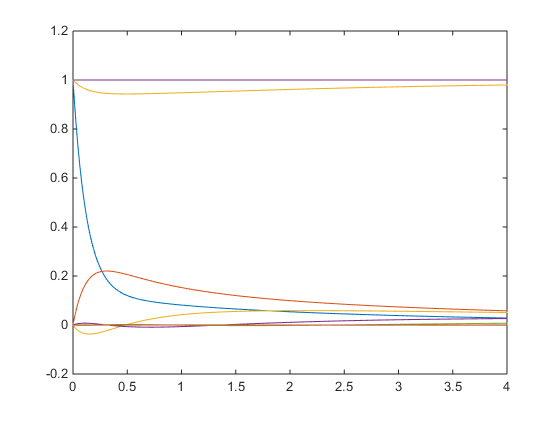
\includegraphics{ode45Trimmed}
      \caption{a = 0, b = 8, N = 9, $k_1=k_2=k_3=k_4=k_5 = 0.5, P_a^T(0) = P_b^R(0) = 1$}
\end{figure}



\end{document}


%\documentclass{article}
\usepackage{amsmath}
\usepackage{bm}
\usepackage{graphicx}
\usepackage[utf8]{inputenc}
\usepackage{caption}
\usepackage{subcaption}
\title{Planning. \\ Mathematical Modelling }
\author{Elisabeth Skaar Hasund}


\begin{document}
\maketitle

\section*{Synaptic cleft in 1D}

Diffusion equation in one dimension

\begin{equation}
u_t = \kappa u_{xx}.
\end{equation}

where $u$ is the concentration of neurotransmitters and $\kappa$ is the diffusion coefficient.

\subsection*{Scaling of variables}

\begin{align*}
\frac{\partial u^*}{\partial t^*} = \kappa \frac{\partial^2u^*}{\partial {x^*}^2}
\end{align*}

Use the scaling 

\begin{align*}
x^* &= L x \\
t^* &= T t \\
u^* &= N u 
\end{align*}

and replace in the diffusion equation s.t.

\begin{align*}
\frac{N}{T}\frac{\partial u}{\partial t} &= \kappa \frac{N^2}{L^2}\frac{\partial^2u}{\partial x^2} \\
\frac{\partial u}{\partial t} &= \eta \frac{\partial^2u}{\partial x^2}, & \eta = \kappa\frac{NT}{L^2}
\end{align*}

Using the values $L = 15 \cdot 10^{-9}$, $T = 10^{-4}$, $N = 5000$ and $\kappa = 0.3\cdot 10^{-12}$, we get the resulting value $\eta \approx 667$. 



\subsection*{Initial and boundary conditions}

The number of neurotransmitters released in one excitation is $N = 5000$. The number of receptor on one membrane is $R \approx \rho_R \cdot \pi r^2 \approx 152$ where $\rho_R$ is the density of receptors and $r$ is the radius of the synaptic cleft. Let $\Omega$ be the line between $0$ and $L$.

Initial values:

\[ u(x,0) = \left\{ 
  \begin{array}{l l}
    N & \text{if x = 0}\\
    0 & \text{elsewhere}
  \end{array} \right.\]

Neumann boundary conditions:

\begin{align*}
u_x(0,t) &= 0, \\
u_x(L,t) &= J(t)
\end{align*}

where $J(t)$ can be thought of as flux describing the rate of reaction in the chemical reaction
\begin{equation}
R + N \rightleftharpoons RN.
\end{equation}

The homogeneous Neumann boundary condition comes from the physical explanation that neurotransmitters cannot go back through the axon terminal.

\subsection*{Numerical scheme}

Using Crank-Nicholsons method, we obtain 

\begin{align*}
(1 - \frac{k}{2h^2} \delta^2_x)U^{n+1}_m = (1 + \frac{k}{2h^2} \delta^2_x) U_m^n
\end{align*}

where $k$ and $h$ are the time and space step, respectively. 

The resulting numerical scheme is

\begin{align*}
\left(I - \frac{r}{2} A\right) U^{n+1} = \left(I + \frac{r}{2} A\right) U^n
\end{align*}

where $r = \frac{k}{h^2}$,


\begin{align*}
A = 
\begin{pmatrix}
  -2 & 1 &  &  \\
  1 & \ddots & \ddots &  \\
    & \ddots  & \ddots & 1 \\
   &  & 1 & -2
\end{pmatrix} 
\textrm{ and }
U = \begin{pmatrix}
U_1 \\
U_2 \\
\vdots \\
U_{M} 
\end{pmatrix}
\end{align*}



Adding Neumann boundary conditions to the system, we expand the numerical scheme to involve boundary points, and an additional term

\begin{align*}
d^n = 
\begin{pmatrix}
0 \\
\vdots \\
0 \\
J^n
\end{pmatrix}
\end{align*}

such that the resulting scheme becomes

\begin{align*}
\left(I - \frac{r}{2} A\right)U^{n+1} = \left(I + \frac{r}{2} A\right) U^n + \frac{k}{2h}(d^n + d^{n+1}).
\end{align*}


\subsection*{Flux}

The rate of Neurotransmitters leaving the synaptic cleft can be described as a flux $J(t)$. Let $\Omega_{\epsilon}$ be a small area close to $L$ with width $\epsilon$, see Figure \ref{fig:model_1d}. Let $N_{\epsilon}(t)$ be the density of neurotransmitters in $\Omega_{\epsilon}$. These neurotransmitters are close enough to react with the receptors, and will affect the flux out of $\Omega$. Let $\rho_R$ be the density of receptors in the area $\epsilon$, and let $P^R(t)$ be the probability that one receptor is available. With reaction constants $k_1$ and $k_2$, the flux can be expressed as

\begin{align*}
J(t) = k_1 N_{\epsilon}(t) \rho_R P^R(t) - k_2 \rho_R (1-P^R(t)).
\end{align*}


\begin{figure}[ht]
        \centering
        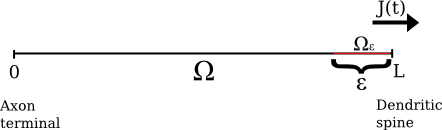
\includegraphics[clip=true,width=0.6\textwidth]{model_1d}
        \caption{Model of the synaptic cleft in one dimension}
        \label{fig:model_1d}
\end{figure}


\section*{Synaptic cleft in 2D}

A 2-dimensional model for the neurotransmitters diffusing from the axon terminal to the dendrite spine.

Let $L$ be the diameter and $b$ the height of the synaptic cleft. Assume that initially the neurotransmitters are uniformly distributed on the axon terminal, and the receptors are uniformly distributed on the dendritic spine. Assume that the surface of the dendritic spine is covered by an extracellular fluid 

CITATION

with thickness $\epsilon$. Like in the 1D-model, the neurotransmitters in this area can react with unoccupied receptors. 

Using the 5-point-formula, one can create a numerical scheme for the diffusion in 2 dimensions. This was attempted, but the system was numerically unstable, so it will not be included in this report. However, Matlab's ODE45 solver was applied to the same problem with success. 

\end{document}


% 2d implementations:
\section{2D diffusion equation}

\subsubsection{Domain, initial and boundary values}

Initially we chose a random point where we released all the neurotransmitters. The initial function for the concentration of neurotransmitters is zero everywhere except from that point. On the boundary we assumed that the particles could freely diffuse outside of the domain.\\
To simplify the diffusion equation we neglect the height of the synaptic cleft. Furthermore, we chose to view the resulting disc as a square with size $4r^2$, due to the difficut nature of the laplacian in cylindrical coordinates. We assume that the receptors are equally distributed over the square.\\If the number of bounded receptor doesn't change over a time interval $\Delta t$, we assume equilibrium and that a signal is being transmitted. \\


\subsubsection{Numerical scheme}
We used the finite difference method to discretize the modelling equations. OBS!(ref.)
$$c_{j,k}^{i+1}=c_{j,k}^{i}+\frac{\Delta t}{2} \Bigg[\kappa \Big(\frac{c_{j+1,k}^{i} -2c_{j,k}^{i} + c_{j-1,k}^{i}}{(\Delta y)^2} +\frac{c_{j,k+1}^{i} -2c_{j,k}^{i} + c_{j,k-1}^{i}}{(\Delta x)^2}\Big)-k_{1}c_{j,k}^i P_{j,k}^i+k_{2}(1-P_{j,k}^i)\Bigg]$$

$$P_{j,k}^{i+1}=P_{j,k}^i + \Delta t \Big[-k_{1}c_{j,k}^iP_{j,k}^i+k_{2}(1-P_{j,k}^i) \Big]$$

\subsubsection{Results}
Using the values given in \cite{fg} with $k_1=10^4$ and $k_2=10$, and 
\begin{itemize}
\item number of steps in x- and y-direction, $nx=ny=10$
\item number of time steps $nt=4\cdot 10^5$, simulated over 1 second
\end{itemize}
This results in a signaling time of $t_s=33.8$ms. The following figures shows the distribution of neurotransmittors and free receptors at the signaling time. 

%results\\
%\begin{figure}
%\begin{subfigure}[b]
%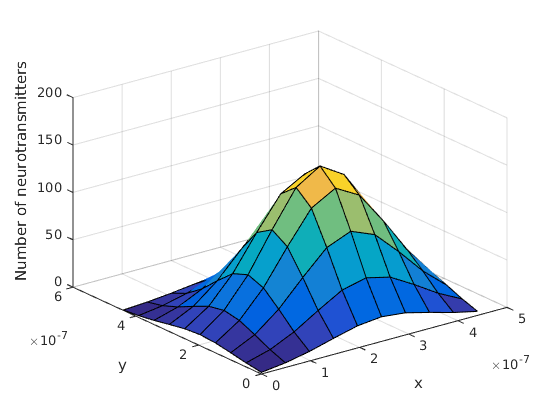
\includegraphics[scale=0.25]{distneurottansmitters}
%\caption{yolo}
%\end{subfigure}
%\begin{subfigure}[b]
%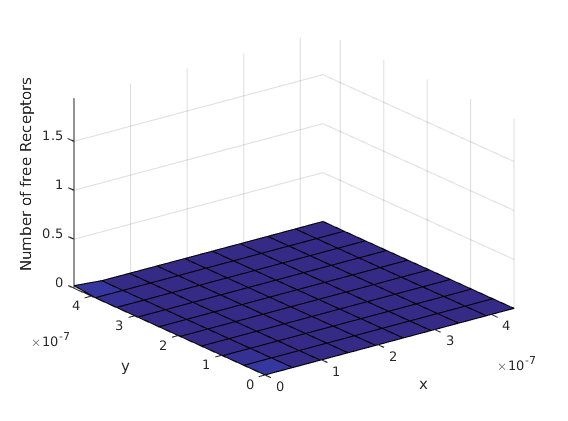
\includegraphics[scale=0.25]{receptordensity}
%\caption{tt}
%\end{subfigure}
%\end{figure}
%
%\begin{figure*}[h!]
%    \centering
%    \begin{subfigure}[b]{0.5\textwidth}
%        \centering
%        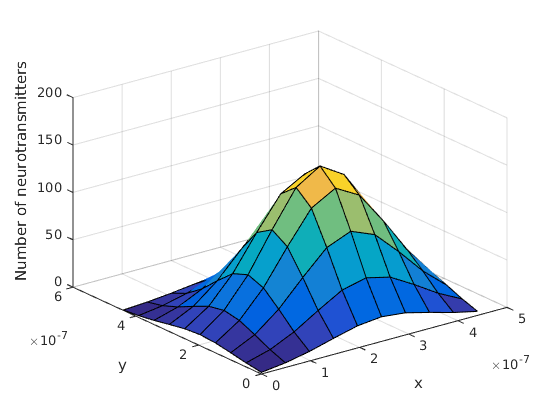
\includegraphics[height=1.2in]{distneurottansmitters}
%        \caption{Neurotransmitters}
%    \end{subfigure}%
%    ~ 
%    \begin{subfigure}[b]{0.5\textwidth}
%        \centering
%        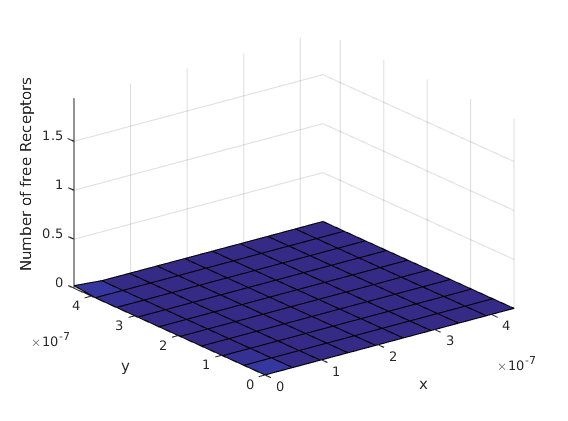
\includegraphics[height=1.2in]{receptordensity}
%        \caption{Receptors}
%    \end{subfigure}
%    \caption{Distribution after a time t=.}
%\end{figure*}


\begin{figure*}[h!]
    \centering
    \begin{subfigure}[b]{0.5\textwidth}
        \centering
        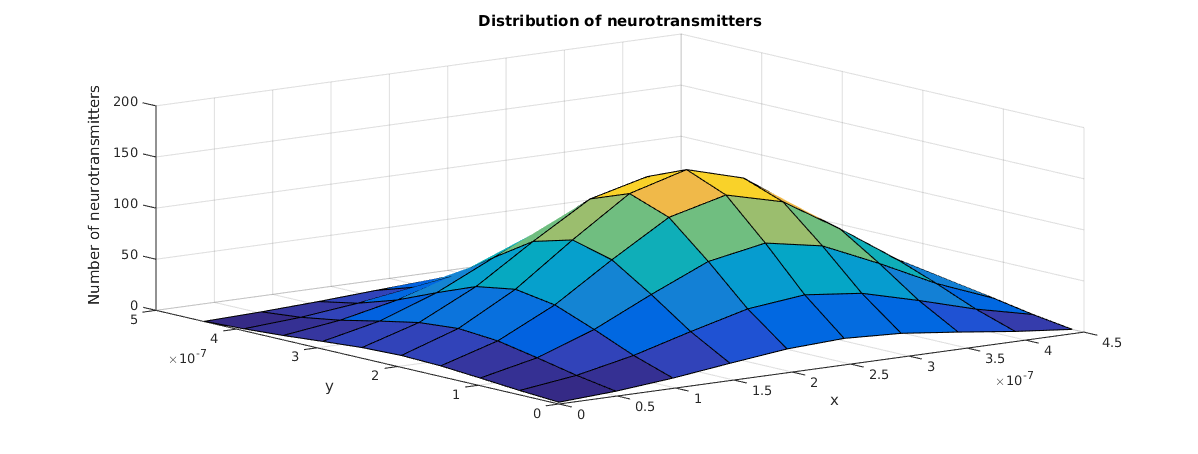
\includegraphics[scale=0.25]{1}
        \caption{Neurotransmitters}
    \end{subfigure}%
    ~ 
    \begin{subfigure}[b]{0.5\textwidth}
        \centering
        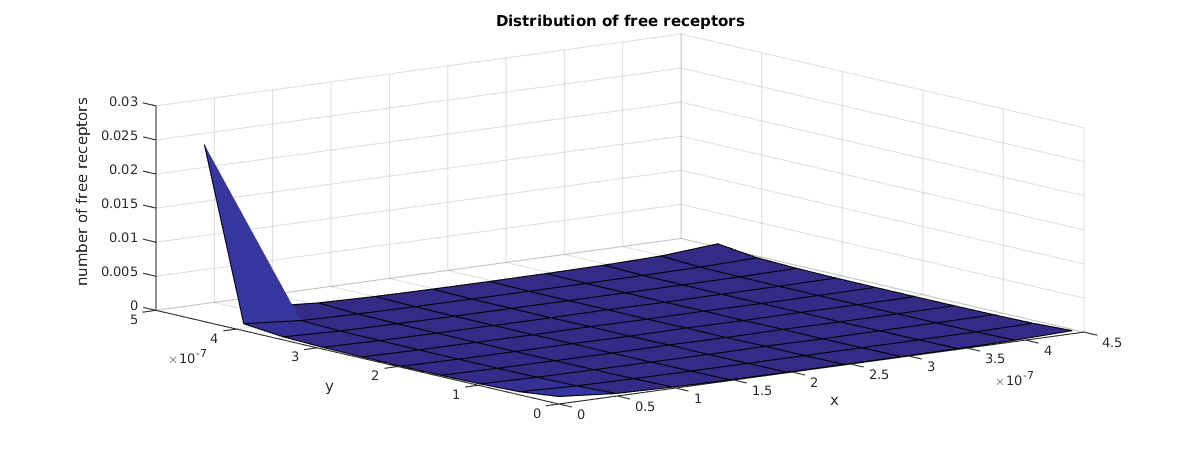
\includegraphics[scale=0.25]{2}
        \caption{Receptors}
        \label{fig1}
    \end{subfigure}
    \caption{Distribution at signal time.}
\end{figure*}

\subsubsection{Discussion}
As we can see from figure \ref{fig1} practically all receptors are bounded at this time, so this may be considered an upper bound for the signaling time. This is a two dimensional model, and thus lacs a certain accuracy. Given more time the model could have been extended to three dimensions, but as a simple representation of what happens during neurotransmission in the synaptic cleft, we consider this model is applicable.\\ Given more time, this model could also have been used to model the clearance time.


\begin{thebibliography}{9}

\bibitem{holstad}
  Jörg Henrik Holstad,
  \emph{Modellering av Diffusjon av Nevrotransmittere
i den Ekstracellulære Væsken}.
  2011.\\
www.duo.uio.no/bitstream/handle/10852/10871\\
/MasteroppgaveHenrikHolstad.pdf \\
Retrieved 13.11.2014


\bibitem{task}
	Xavier Raynaud,
	\emph{TMA4195 - Mathematical modeling (Fall 2014).
Project descriptions.}\\
www.math.ntnu.no/emner/TMA4195/2014h/public/project.pdf\\
Retrieved 13.11.2014


\end{thebibliography}



\end{document}
